\section[Desenvolvimento do Projeto]{Desenvolvimento do Projeto}

\subsection{Repositório do Código Fonte do Projeto}
  No projeto, organizamos os materiais em repositórios separados para \href{https://tools.ages.pucrs.br/uma-porto-alegre-alem/frontend}{\textit{frontend}}, \href{https://tools.ages.pucrs.br/uma-porto-alegre-alem/backend}{\textit{backend}} e \href{https://tools.ages.pucrs.br/uma-porto-alegre-alem/wiki}{\textit{wiki}}, o que facilitou bastante o acompanhamento das entregas e a divisão das responsabilidades entre os times. Na \textit{wiki}, centralizamos os links e a documentação principal para manter o contexto técnico acessível para todos, incluindo decisões de arquitetura, organização das tarefas e alinhamentos com os clientes.

  Também estruturamos o trabalho com foco em rastreabilidade, conectando \textit{user stories}, tarefas técnicas e entregas por sprint. Essa organização foi importante para eu conseguir acompanhar o que estava pendente no painel administrativo, no gerenciamento das edificações e nos fluxos ligados a idiomas e mídias, sem perder a visão do produto como um todo. Para isso, utilizamos o \textit{board} do GitHub Projects.

\subsection{Banco de Dados Utilizado}
  O banco de dados principal escolhido para o projeto foi o MongoDB Atlas \cite{mongodbatlas}. A decisão fez sentido para o nosso contexto porque o produto precisa lidar com conteúdos variados e com possibilidade de evolução frequente, como informações de edificações, materiais multimídia e dados administrativos.

  Como o MongoDB Atlas é um serviço gerenciado, ele também ajudou a reduzir esforço operacional com manutenção, backup e disponibilidade. Na prática, isso nos permitiu focar mais na modelagem dos dados e nas regras de negócio do sistema, em vez de gastar energia com configuração de infraestrutura de banco do zero.

\begin{figure}[H]
    \centering
    \small
    \caption{Diagrama do Banco de Dados}
    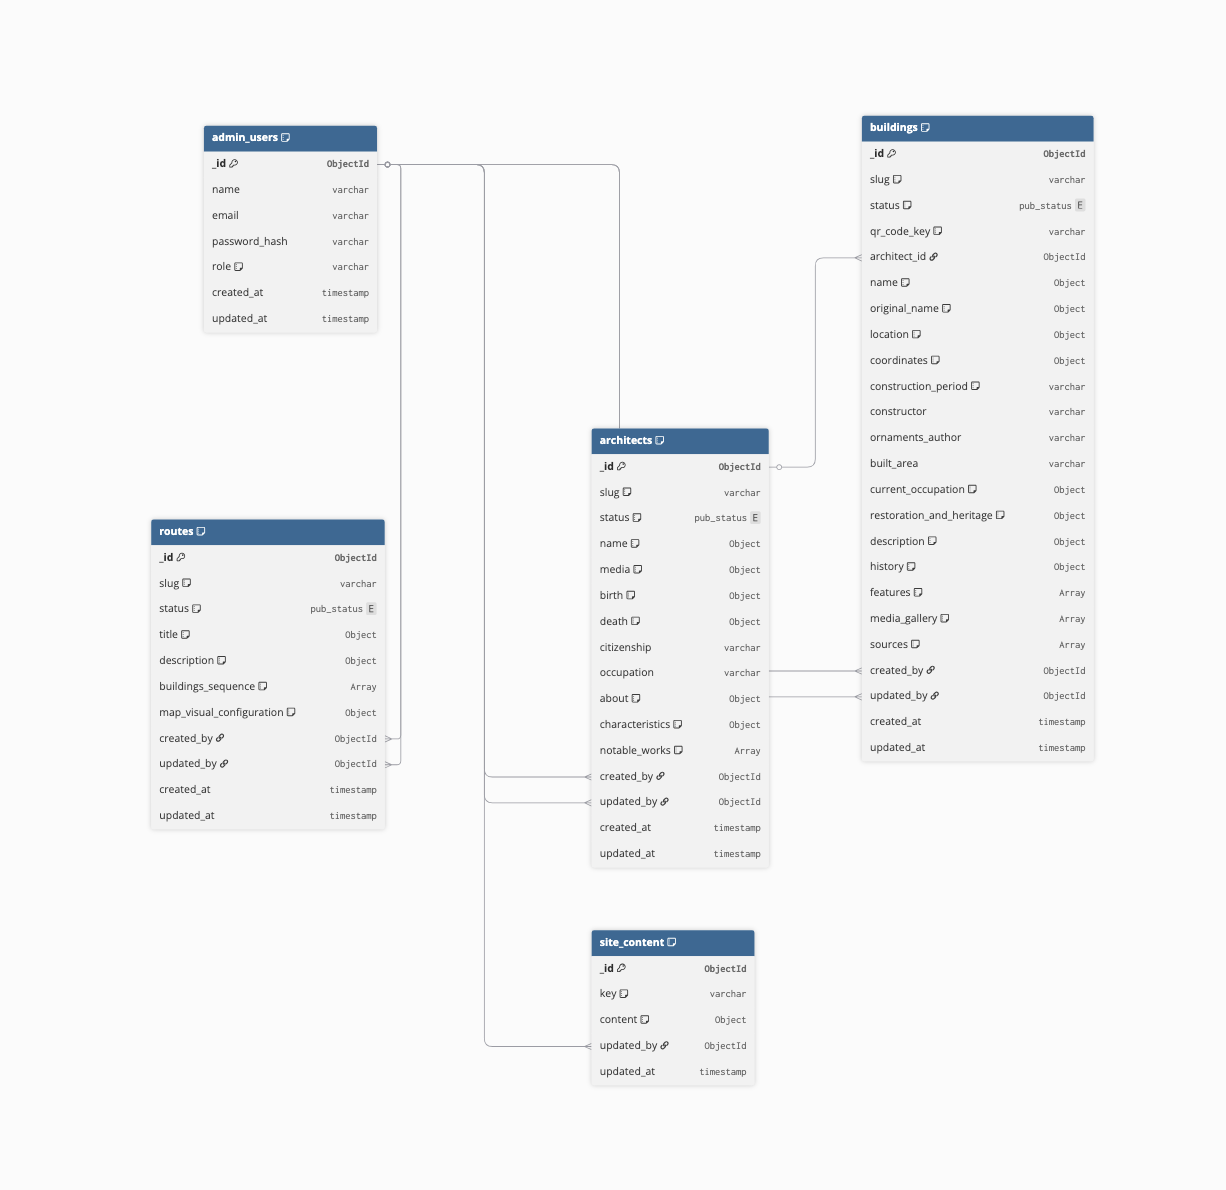
\includegraphics[width=1\linewidth]{conteudo/5 - ages IV/conteudo/figures/DiagramaBancoUmaPortoAlegreAlema.png}

    Fonte: Diagrama feito pelos AGES II.
    \label{fig:diagrama-banco-uma-porto-alegre-alema}
\end{figure}

\subsection{Arquitetura Utilizada}
  A arquitetura do sistema foi definida em três camadas: \textit{frontend}, \textit{backend} e dados/armazenamento. No \textit{frontend}, utilizamos o \ac{aws} Amplify \cite{awsamplify} para publicar a aplicação web com \textit{deploy} automatizado a partir do repositório. No \textit{backend}, adotamos NestJS \cite{nestjs} em \textit{container} Docker \cite{docker} rodando no \ac{ecs} Fargate \cite{awsecs,awsfargate}, o que simplificou a operação por não exigir gerenciamento direto de servidores.

  Na camada de dados e arquivos, utilizamos MongoDB Atlas para persistência principal e Amazon \ac{s3} \cite{awss3} para armazenamento de imagens, áudios e documentos. Para proteger informações sensíveis, como credenciais e chaves, utilizamos \ac{aws} Secrets Manager \cite{awssecretsmanager}. Esse desenho trouxe um bom equilíbrio entre simplicidade, segurança e escalabilidade, além de facilitar a evolução da plataforma conforme novas demandas do projeto cultural surgirem.

  Em termos de fluxo, o usuário acessa o \textit{frontend} no navegador, que envia requisições para a \ac{api}. O \textit{backend} processa essas requisições e, quando necessário, consulta o MongoDB, manipula arquivos no \ac{s3} e busca segredos no Secrets Manager. Depois disso, a resposta retorna ao \textit{frontend} para exibição ao usuário final. A Figura~\ref{fig:arquitetura-ages-iv} apresenta a organização planejada para essa arquitetura. A solução final ainda não está implementada, então seguimos com a arquitetura planejada para garantir que o desenvolvimento fique alinhado com as necessidades do projeto e dos \textit{stakeholders}.

\begin{figure}[H]
    \centering
    \small
    \caption{Arquitetura do Projeto}
    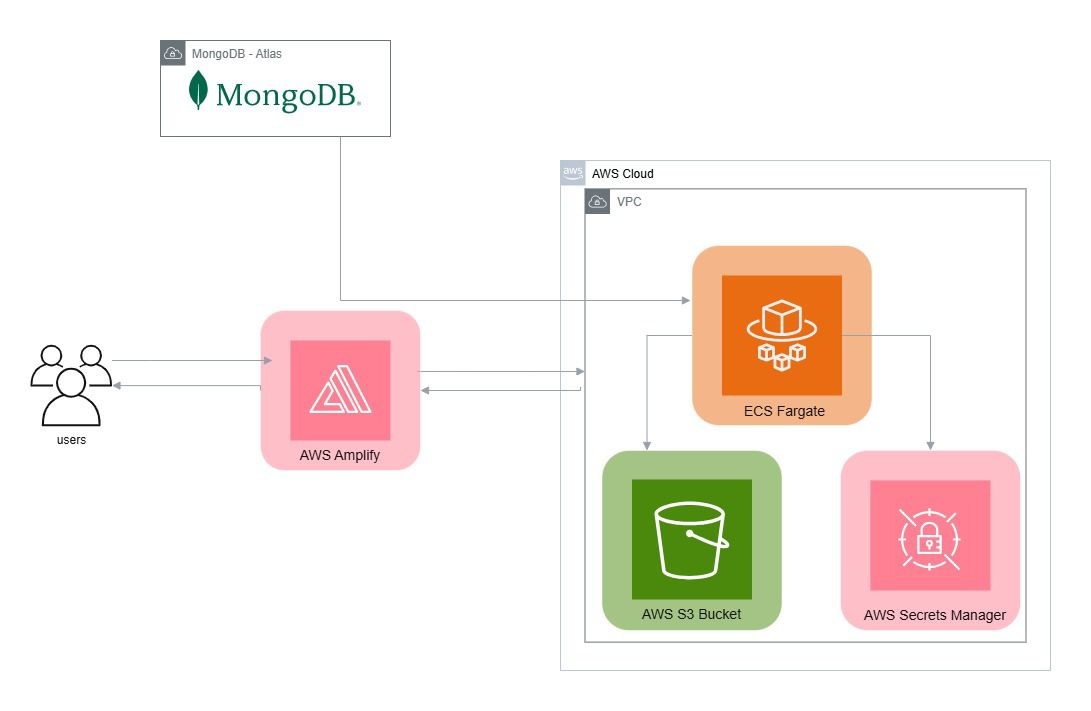
\includegraphics[width=1\linewidth]{conteudo/5 - ages IV/conteudo/figures/arquitetura-agesIV.jpeg}

    Fonte: documentação do projeto
    \label{fig:arquitetura-ages-iv}
\end{figure}

\subsection{Protótipos das Telas Desenvolvidas}
  Os protótipos foram desenvolvidos no Figma \cite{figma} e foram parte crucial para alinhar a visão do produto entre os \textit{stakeholders} e o time de desenvolvimento. Eles ajudaram a definir a estrutura das páginas, a navegação e a organização dos conteúdos, além de facilitar o \textit{feedback} e as iterações durante o processo de design. A seguir, apresentamos exemplos de protótipo para ilustrar a proposta visual do \textit{website}:

\begin{figure}[H]
    \centering
    \small
    \caption{Protótipo no Figma - Landing Page}
    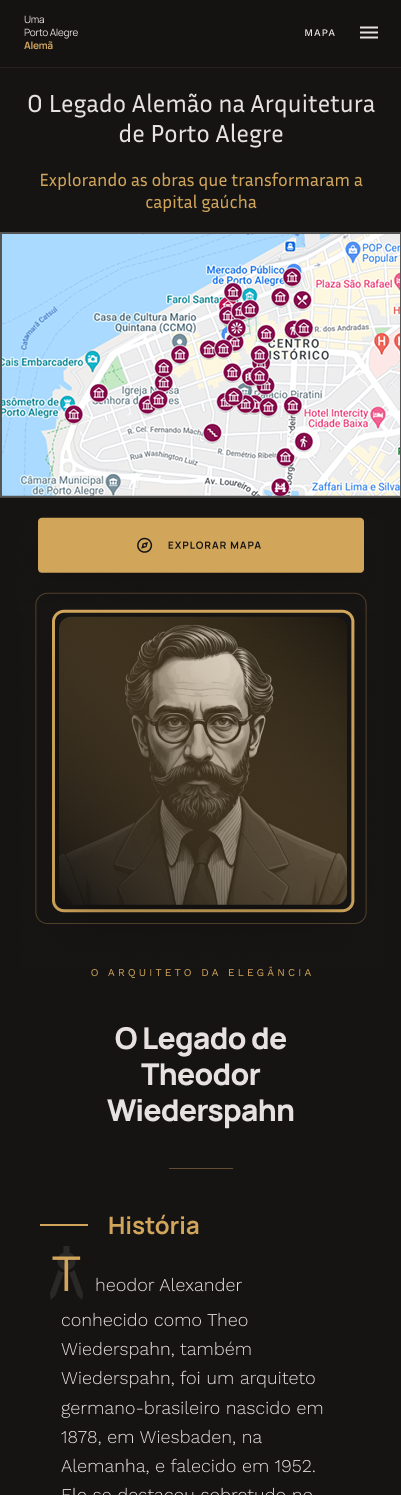
\includegraphics[width=0.50\linewidth,height=0.75\textheight,keepaspectratio]{conteudo/5 - ages IV/conteudo/figures/LandingPage.png}

    Fonte: Figma do projeto
    \label{fig:figma-landing-ages-iv}
\end{figure}

\begin{figure}[H]
    \centering
    \small
    \caption{Protótipo no Figma - Mapa}
    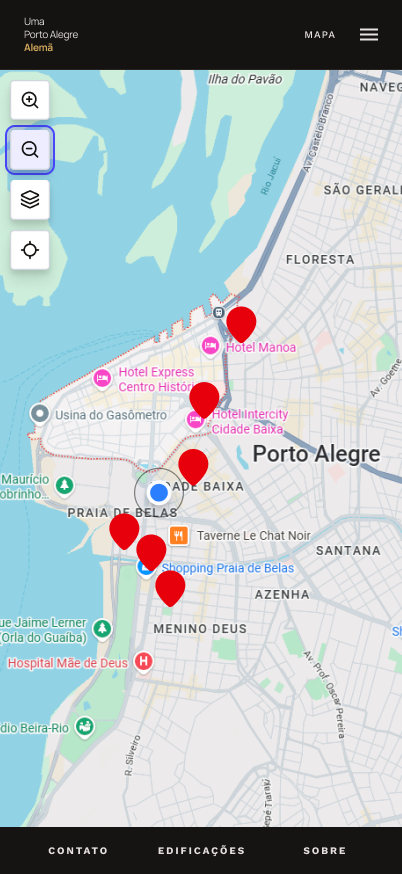
\includegraphics[width=0.50\linewidth,height=0.75\textheight,keepaspectratio]{conteudo/5 - ages IV/conteudo/figures/Mapa.png}

    Fonte: Figma do projeto
    \label{fig:figma-mapa-ages-iv}
\end{figure}

\begin{figure}[H]
    \centering
    \small
    \caption{Protótipo no Figma - Detalhe no Mapa}
    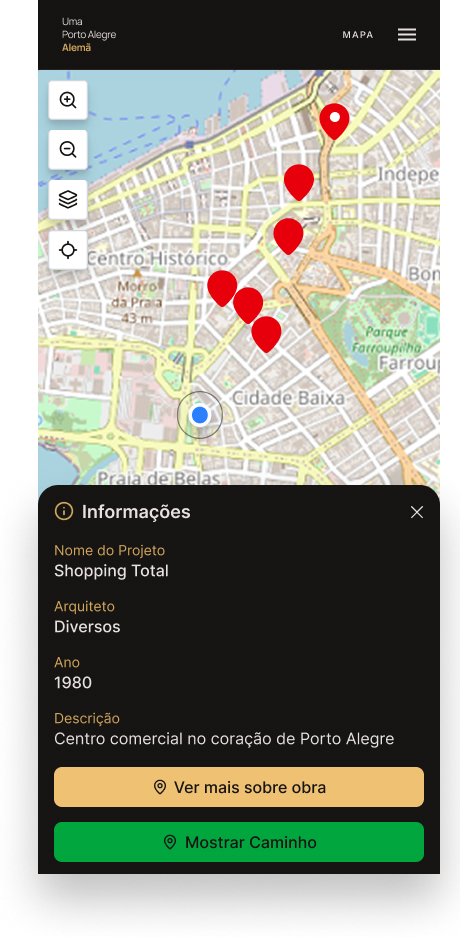
\includegraphics[width=0.50\linewidth,height=0.75\textheight,keepaspectratio]{conteudo/5 - ages IV/conteudo/figures/DetalheNoMapa.jpg}

    Fonte: Figma do projeto
    \label{fig:figma-detalhe-mapa-ages-iv}
\end{figure}

\begin{figure}[H]
    \centering
    \small
    \caption{Protótipo no Figma - Detalhe de Edificações}
    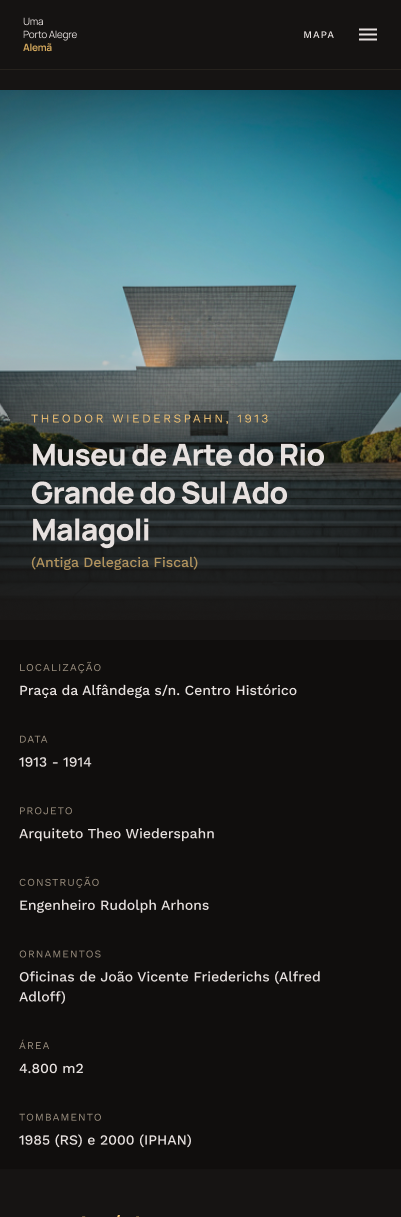
\includegraphics[width=0.50\linewidth,height=0.75\textheight,keepaspectratio]{conteudo/5 - ages IV/conteudo/figures/DetalheEdificacoes.png}

    Fonte: Figma do projeto
    \label{fig:figma-detalhe-edificacoes-ages-iv}
\end{figure}

\subsection{Tecnologias Utilizadas}
  A base de desenvolvimento do projeto foi definida com TypeScript \cite{typescript} tanto no \textit{frontend} quanto no \textit{backend}. Essa escolha ajudou a manter maior consistência entre as camadas da aplicação, reduzir erros de tipagem e facilitar a manutenção do código ao longo das sprints.

  No \textit{frontend}, utilizamos React \cite{react} com Next.js \cite{nextjs}, combinação que nos permitiu estruturar melhor a interface do \textit{website}, organizar rotas de forma mais clara e evoluir as telas com boa reutilização de componentes. No \textit{backend}, utilizaremos NestJS, que trouxe uma estrutura modular alinhada com o padrão que queríamos para o \ac{cms} e para as \ac{api}s do projeto. No geral, essa \textit{stack} focada em TypeScript, React/Next.js e NestJS deixou o desenvolvimento mais coeso entre \textit{frontend} e \textit{backend} e diminuiu a curva de aprendizado para o time, já que utilizamos as mesmas linguagens e conceitos em ambas as camadas.
  
